\section{Applications for Single Graph Data}\label{sec:single_app}
In this section, we explore the applications of the single graph models in Section \ref{sec:single_graph_models} and the algorithms in Section \ref{sec:single_algo}. The \textit{Drosophila} mushroom body connectome and HCP data are analyzed (see Appendix \ref{sec:drosphila} and \ref{sec:hcp} for description) along with simulated examples, and Appendix \ref{sec:single_app_appendix} contain additional analysis in weighted connectomes. 

\subsection{Testing for Differences Between Communities of Edges}
\label{sec:sg_dros_siem}

In Figure \ref{fig:siem_uwt}, we compare a number of different strategies using Fisher's exact test \cite{fisher1925statistical} for testing whether there exists a difference between $K=2$ communities, or groups, of edges in a graph. Formally, let $e_{ij}^{(k)} \sim F_k$ be a single edge in the graph, where $k \in\left\{ 1, 2\right\}$ is a community of edges, for $i, j \in [n]$. Our hypothesis test of interest is:
\begin{align*}
    H_0: F_1 = F_2, \quad
    H_a: F_1 \neq F_2
\end{align*}
We simulate graphs from the homophilic planted partition $\sbm$  from Section \ref{sec:usbm} and symmetric homotopic $\siem$ from Section \ref{sec:usiem} in Figure \ref{fig:siem_uwt}a(i). Under the given models, our hypotheses simplify to testing whether $p_1 = p_2$ against $p_1 \neq p_2$; that is, whether or not there exists a different probability for each edge community. Effect size, or the difference in probability between the two communities, for the $\sbm$ and the $\siem$ are varied linearly from $0$ to $0.1$, and from $0$ to $0.5$, respectively. 
% Under the null, the distributions $F_1, F_2$ of the two communities are identical, and under the alternative, the two distributions are different. 
A relative effect size of $0$ corresponds to an $\er$ graph, in which $F_1 = F_2$; at all other relative effect sizes, the alternative is true. We measure performance using the statistical power at $\alpha = 0.05$ in Figure \ref{fig:siem_uwt}a(ii). Across the simulation settings, we see that Fisher's exact test provides an appropriate statistical test and provides sufficiently high  power with large enough effect size and graph. Importantly, Fisher's test displays  both empirical validity (at an effect size of zero, the power is at most $\alpha$) and empirical consistency (the test power converges to $1$ as the effect size increases) in both simulations.

We demonstrate our techniques developed above on the \textit{Drosophila} mushroom body, with $n=319$ vertices in the left or right hemisphere (2 vertices located along the center of the brain are excluded). In Figure \ref{fig:siem_uwt}b we investigate the appropriateness of different unweighted independent edge models for the \textit{Drosophila} mushroom body. Our goal is to identify whether the unweighted \textit{Drosophila} mushroom body display homophilia (that is, the within hemisphere blocks have greater connectivity than between hemisphere blocks) or homotopia (that is, edges incident bilateral vertices have a different distribution from edges incident non-bilateral vertices). Figure \ref{fig:siem_uwt}b(i) shows the unweighted \textit{Drosophila} mushroom body. The within-hemisphere blocks appear to have a higher proportion of edges than the between-hemisphere edge blocks, shown in Figure \ref{fig:siem_uwt}b(ii). There is strong evidence that the within-hemisphere connectivity exceeds the between-hemisphere connectivity (Fisher's exact test, $p$-value=$0.0$). Next, we investigate whether the graph is homotopic; that is, whether bilateral (homotopic) connectivity exceeds non-bilateral (heterotopic) connectivity, in Figure \ref{fig:siem_uwt}b(iii). Strong evidence is present that homotopic connectivity exceeds heterotopic connectivity (Fisher's exact test, $p$-value=$0.0$).

Finally, we explore the appropriateness of various independent edge models for diffusion connectomes from the HCP Dataset. The diffusion connectomes are binarized according to whether an edge is present (the edge weight is greater than zero) or absent (the edge weight is zero). Figure \ref{fig:siem_uwt}c(i) shows the average unweighted diffusion connectome over all participants in the study. Figure \ref{fig:siem_uwt}c(ii) shows the distribution of edge-weights within-hemisphere versus between-hemisphere. The diffusion connectomes appear to possess homophily; i.e., high within-hemisphere connectivity, with lower between-hemisphere connectivity. This is demonstrated by the fact that in all $N$=$1059$, the within-hemisphere connectivity exceeds the between-hemisphere connectivity. This effect can be observed by looking at the difference between within-hemisphere connectivity and between-hemisphere connectivity for each of the $N=1059$ connectomes, shown in \ref{fig:siem_uwt}c(iii). All $1059$ diffusion connectomes have significantly higher within-hemisphere connectivity than between-hemisphere connectivity at $\alpha=.05$ after Bonferroni correction (Fisher's exact test, $N=1059$, maximum $p$-value$<10^{-20}$).

\begin{figure}
    \centering
    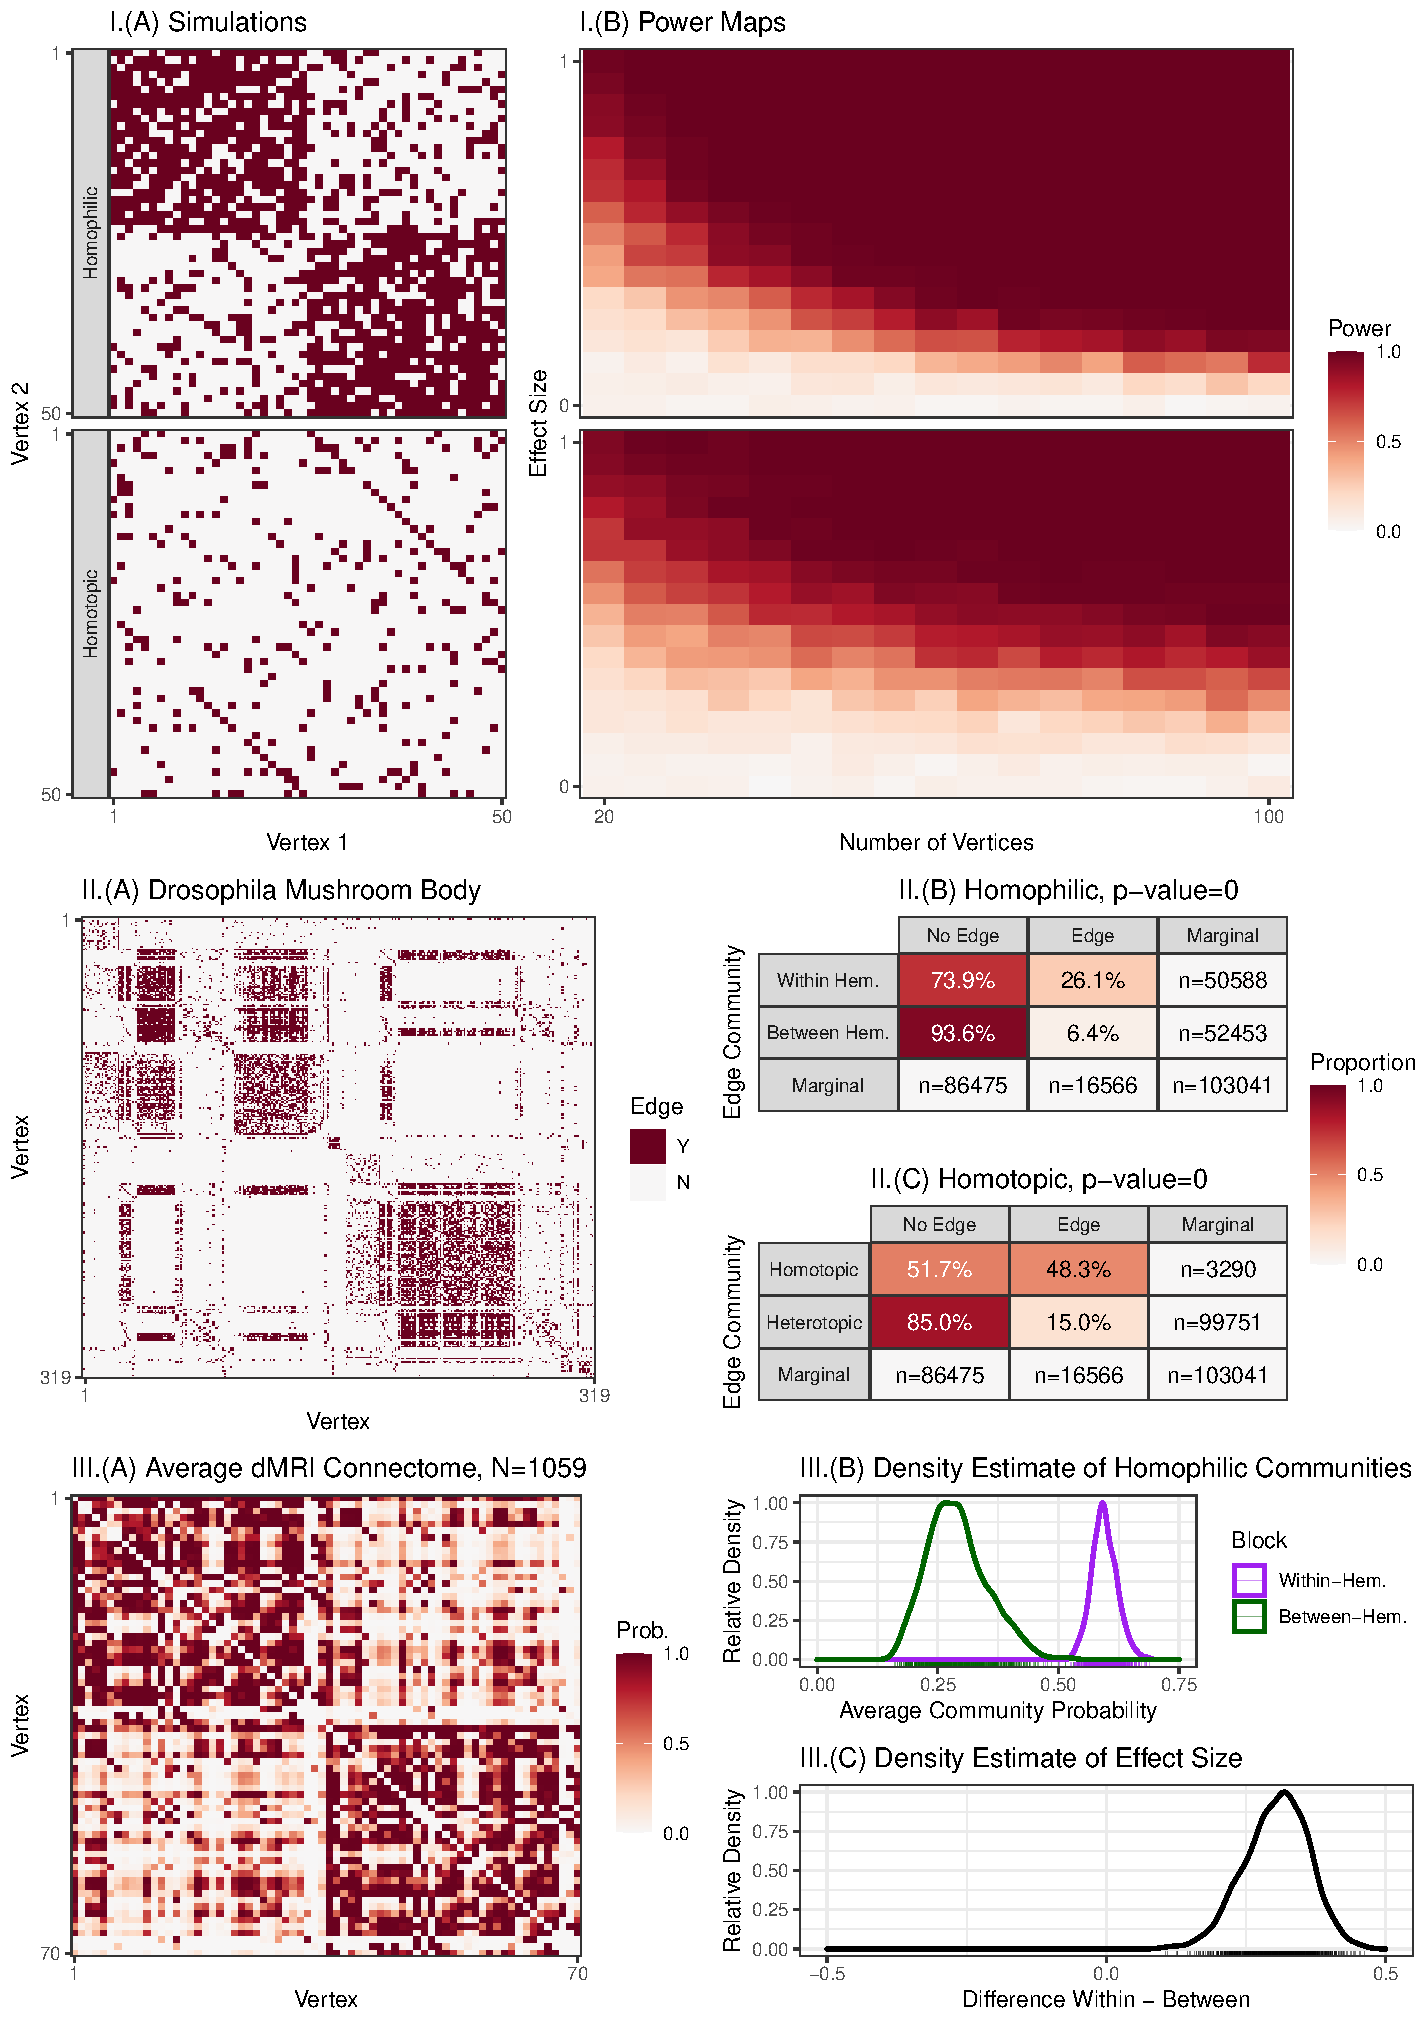
\includegraphics[width=.9\linewidth]{figures/dnd/siem_figure.pdf}
    \caption
    [Comparing communities of edges in graphs.]
    {\textbf{Comparing communities of edges in graphs}. \textbf{a(ii)} Fisher's exact test shows reasonable statistical power across both homophilic and homotopic block structures in \textbf{a(i)}, with power converging to $1$ as effect size and number of vertices grow. \textbf{b(ii)} and \textbf{b(iii)} the \textit{Drosophila} mushroom body in \textbf{b(i)} shows both homophilic planted partition and homotopic structure (Fisher's exact test, $p$-values$=0$). \textbf{c(ii)} and \textbf{c(iii)} all $N=1059$ Human Connectome Project (HCP) diffusion connectomes show homophilic planted partition structure, with within-hemisphere connectivity exceeding between-hemisphere connectivity (Fisher's exact test, $N=1059$, Bonferroni corrected $p$-values$<10^{-21}$).}
    \label{fig:siem_uwt}
\end{figure}

Appendix \ref{sec:siem_wt} investigates the fit of independent edge models for weighted graphs from the \textit{Drosophila} mushroom body and the HCP diffusion connectomes. We leverage the Mann-Whitney Wilcoxon Test, a non-parametric test of whether there exists a difference in medians between the two edge-clusters. We again find that the weighted \textit{Drosophila} mushroom shows both homotopic planted partition structure and homophily, and that the weighted HCP connectomes all show homotopic planted partition structure ($N$=$1059$), a conclusion consistent with our results on the unweighted graphs. 

\subsection{Model Selection for Appropriate Block Structure}
\label{sec:sbm_block_est}

Recall that in Section \ref{sec:usbm}, that for the case of a $K=2$ $\sbm$, the matrix $\B$ with entries $\B_{kl}$ defines the probability of an edge connecting a vertex in community $k$ with a vertex in community $l$. By the bias-variance trade-off, simply supposing a unique entry for each block of $\B$ adds an additional level of complexity to the model, and may reduce the quality of inference, so the ability to make a principled decision when faced with numerous potential block structures is of importance. Formally, we are concerned with choosing one of the appropriate block structures from a subset of candidate block structures given in Section\ref{sec:usbm}, presenting a problem in model selection. Our hypotheses are the alternate candidate models, and our goal is to select the hypothesis corresponding to the candidate model that is most supported by the data by using the model with the lowest $p$-value.

In Figure \ref{fig:sbm_uwt}a, we perform simulations where the true graph is either $\er$, Planted Partition, and Symmetric Heterogeneous, as shown in Figure \ref{fig:sbm_uwt}a(i). Effect size corresponds to the magnitude of the difference between disparate blocks in the model. We find that the $\chi^2$ test 
is an appropriate test for identification of block structure in unweighted graphs, and successfully recovers the correct block structure as the effect size and the number of vertices increases. Figure \ref{fig:sbm_uwt}a(ii) shows the test features both empirical validity and empirical consistency, as in Figure \ref{fig:siem_uwt}. 
% Performance is worst for the Asy. Het. example, when each block has its own unique probability.

In Figure \ref{fig:sbm_uwt}b, we investigate the appropriate block structure for the unweighted \textit{Drosophila} mushroom body, which is shown in  shows the probability of an edge existing within each block of $\B$, where the $n=319$ vertices in either the left or right hemisphere are partitioned according to hemisphere. 
% TODONE 'it would appear'? is this a soap opera? just state the results please ;)
% phantom of the opera actually :D --eb
The on-diagonal (Left,Left) and (Right,Right) blocks share a similar distribution that is unique from the (Left, Right) and (Right, Left) blocks. Because the \textit{Drosophila} mushroom body is inherently a directed graph, we investigate whether it is $\er$, Planted Partition, Asymmetric Homogeneous, Symmetric Heterogeneous, or Asymmetric Heterogeneous, using the $\chi^2$ test. Testing indicates that the \textit{Drosophila} mushroom body possesses a planted partition structure ($\chi^2$ test, $p$-value=$0.0$). 
% TODONE what does 'the best fit model is to assume symmetic ....' mean? maybe state p-values for each test?
This has the interpretation that the optimal $\sbm$ includes a shared probability for the on-diagonal (Left,Left) and (Right,Right) blocks, and a different shared probability for the off-diagonal (Left,Right) and (Right,Left) blocks. An important considerations is that while the optimal $\sbm$ is symmetric, the graph itself is directed. This has the implication that while the $\sbm$ would posit that edges in the (Left,Right) and (Right,Left) blocks have the same probability, realizations of the (Left,Right) and (Right,Left) block will not necessarily be identical. 

Figure \ref{fig:sbm_uwt}c investigates the optimal block structure for the $N$=$1059$ diffusion connectomes from the HCP dataset. The figure shows the average connectivity for the $3$ possible unique entries of the block probability matrix $\B$ for an $\sbm$ where vertices are segmented into communities according to hemisphere: Left-Hemisphere Connectivity, Right-Hemisphere Connectivity, and Contralateral (between-hemisphere) connectivity. Because the diffusion connectomes are inherently symmetric, the graph is directionless, and hence it is not possible for the \textit{Left, Right} and \textit{Right, Left} blocks to have different values. We consider $3$ possible block structures for the diffusion connectome: $\er$, Planted Partition, and Symmetric Heterogeneous. On all $N$=$1059$ connectomes, the optimal block structures is Planted Partition, using the $\chi^2$ test.

Appendix \ref{sec:sbm_est_wt} proposes the use of several testing variants (ANOVA, Kruskal-Wallis, and Distance Correlation) for the weighted drosophila mushroom body and the weighted HCP diffusion connectomes for investigating the optimal block structure. All tests yield the same conclusion (and in the case of the HCP dataset, again for all $N$=$1059$ connectomes) that the mushroom body and diffusion connectomes display planted partition structure. An important consideration is that the implication for weighted graphs is, rather than the on-diagonal and off-diagonal blocks sharing the same probability (as is the case for the unweighted graphs), the 2 on-diagonal blocks (\textit{Left, Left} and \textit{Right, Right}) share a \textit{common distribution}. The implication is similar for the 2 off-diagonal blocks (\textit{Left, Right} and \textit{Right, Left}).

\begin{figure}
    \centering
    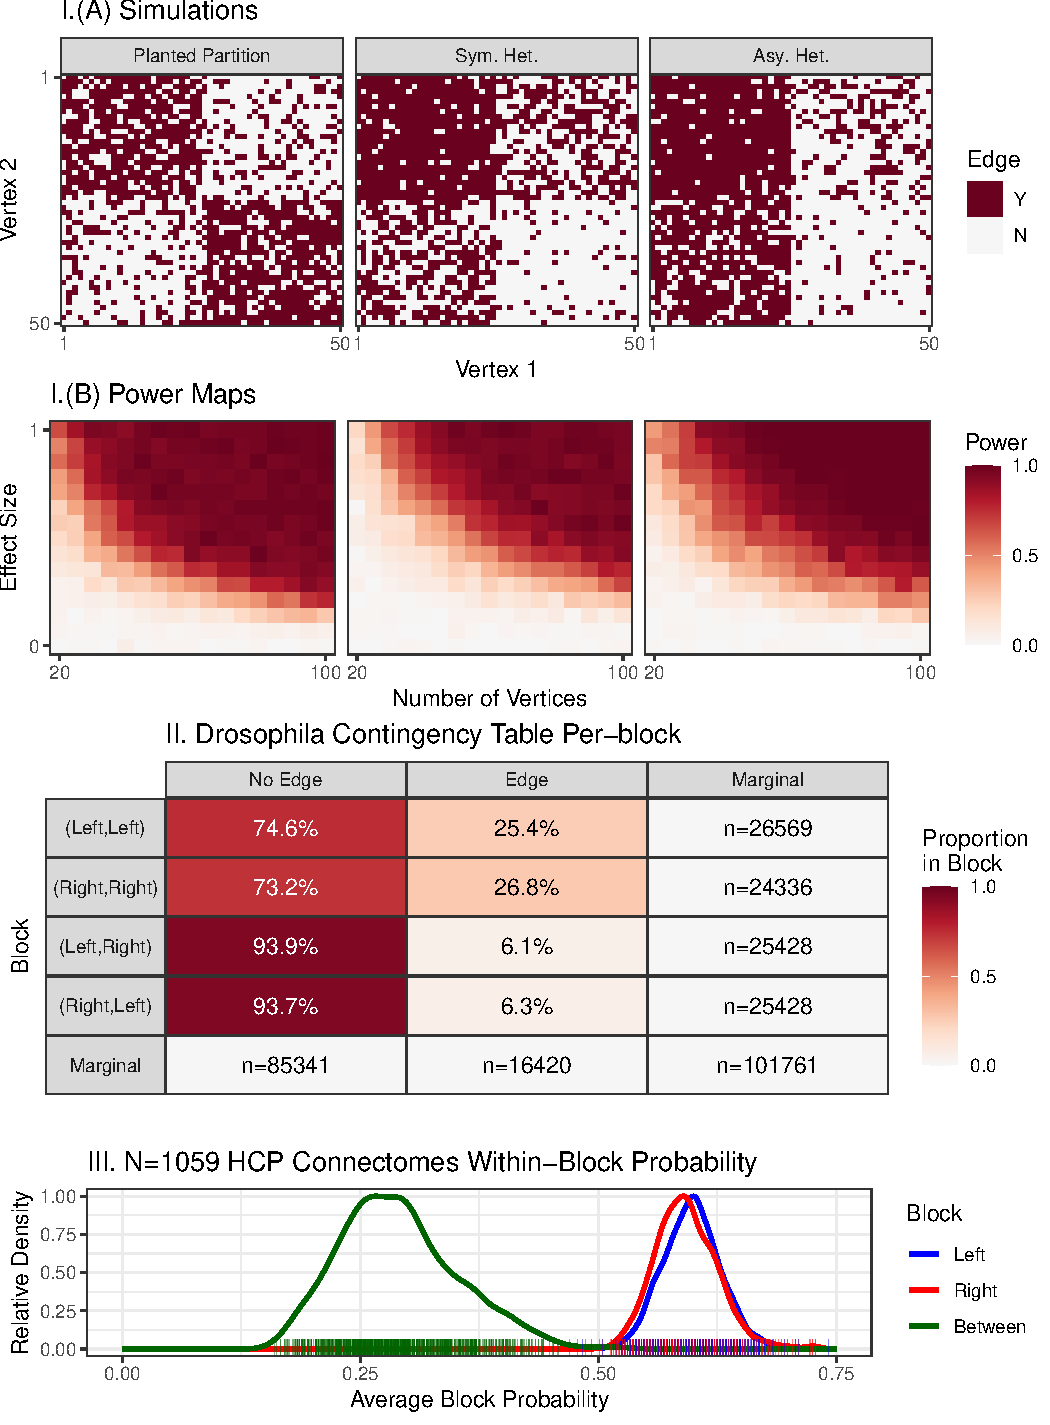
\includegraphics[width=.8\linewidth]{figures/dnd/sbm_uwt.pdf}
    \caption
    [Estimating optimal block structure.]
    {\textbf{Estimating optimal block structure}. \textbf{a(ii)} $\chi^2$ test is effective for identifying the ideal block structure across disparate candidate block structures from \textbf{a(i)}, as power improves as both effect size and graph size increase. \textbf{b.} The \textit{Drosophila} mushroom body displays a planted partition structure ($\chi^2$ test, $p$-value=$0.0$), where \textit{(Left, Left)} and \textit{(Right, Right)} blocks share a different probability from the \textit{(Left, Right)} and \textit{(Right, Left)} blocks. \textbf{c.} Similarly, all $N=1059$ Human Connectome Project (HCP) diffusion connectomes show planted partition structure, with a similar interpretation to the \textit{Drosophila} result.}
    \label{fig:sbm_uwt}
\end{figure}


\subsection{Same Network, Different Communities}
In the case of 2-block $\sbm$s with positive semi-definite block probability matrix $\B = [a, b;b,c]$, there are two structures of interest: affinity and core-periphery. In affinity structure, $a, c \gg b$, that is the within-block connectivity is relatively higher than that of between-block connectivity. In the core-periphery structure, $a \gg b, c$, that is one block has relatively higher within-block connectivity than those of other block's within-block probability and between-block connectivity.

In this section, we examine the two spectral embedding clustering approaches described in Section \ref{sec:ase} which produce different clusterings depending on the $\sbm$ model \cite{priebe2019two, cape2019spectral}. In short, $\ase$ clustering tends to favor core-periphery structure while $\lse$ clustering tends to favor affinity structure.

We consider graphs generated from 4-block $\sbm$ with $n=4000$ vertices, membership vector $\vec{\pi} = [0.25, 0.25, 0.25, 0.25]$, and the block probability matrix
\begin{align*}
    \mathbf{B} = 
    \begin{blockarray}{ccccc}
        & A & B & C & D \\
        \begin{block}{c[cccc]}
        A & 0.01 & 0.02  & 0.01   & 0.002 \\
        B & 0.02 & 0.1   & 0.002  & 0.015  \\
        C & 0.01 & 0.002 & 0.01  & 0.02 \\
        D & 0.002 & 0.015 & 0.02 & 0.01 \\
        \end{block}
    \end{blockarray}
\end{align*}
The above 4-block $\sbm$ exhibit both affinity and core-periphery structures when projected down to 2-blocks, which are shown below:
\begin{align*}
    \mathbf{B}_{affinity} \approx 
    \begin{blockarray}{ccc}
        & AB & CD  \\
        \begin{block}{c[cc]}
        AB & 0.04 & 0.007  \\
        CD & 0.007 & 0.04  \\
        \end{block}
    \end{blockarray},~ &
    \mathbf{B}_{core} \approx
    \begin{blockarray}{ccc}
        & AC & BD  \\
        \begin{block}{c[cc]}
        AC & 0.01 & 0.01  \\
        BD & 0.01 & 0.06  \\
        \end{block}
    \end{blockarray}
\end{align*} 
Blocks $AB$ and $CD$ form $B_{affinity}$, which exhibit the affinity structure, while blocks $AC$ and $BD$ form $B_{core}$, which exhibit the core-periphery structure. 
A network is sampled from the 4-block $\sbm$ model, and spectral clustering is performed (see Section \ref{sec:clustering_single}) with embedding dimension $\hat d=2$ and $K=2$ number of clusters. Figure \ref{fig:exp8} shows the spectral clustering results. In panel \ref{fig:exp8}a, clustering with $\lse$ shows the blocks forming affinity structures are grouped together, and, in panel \ref{fig:exp8}b, clustering with $\ase$ shows the blocks forming core-periphery structures grouped together. Thus, the two different spectral clustering methods provide two different groups that are both meaningful. 

\begin{figure}
    \centering
    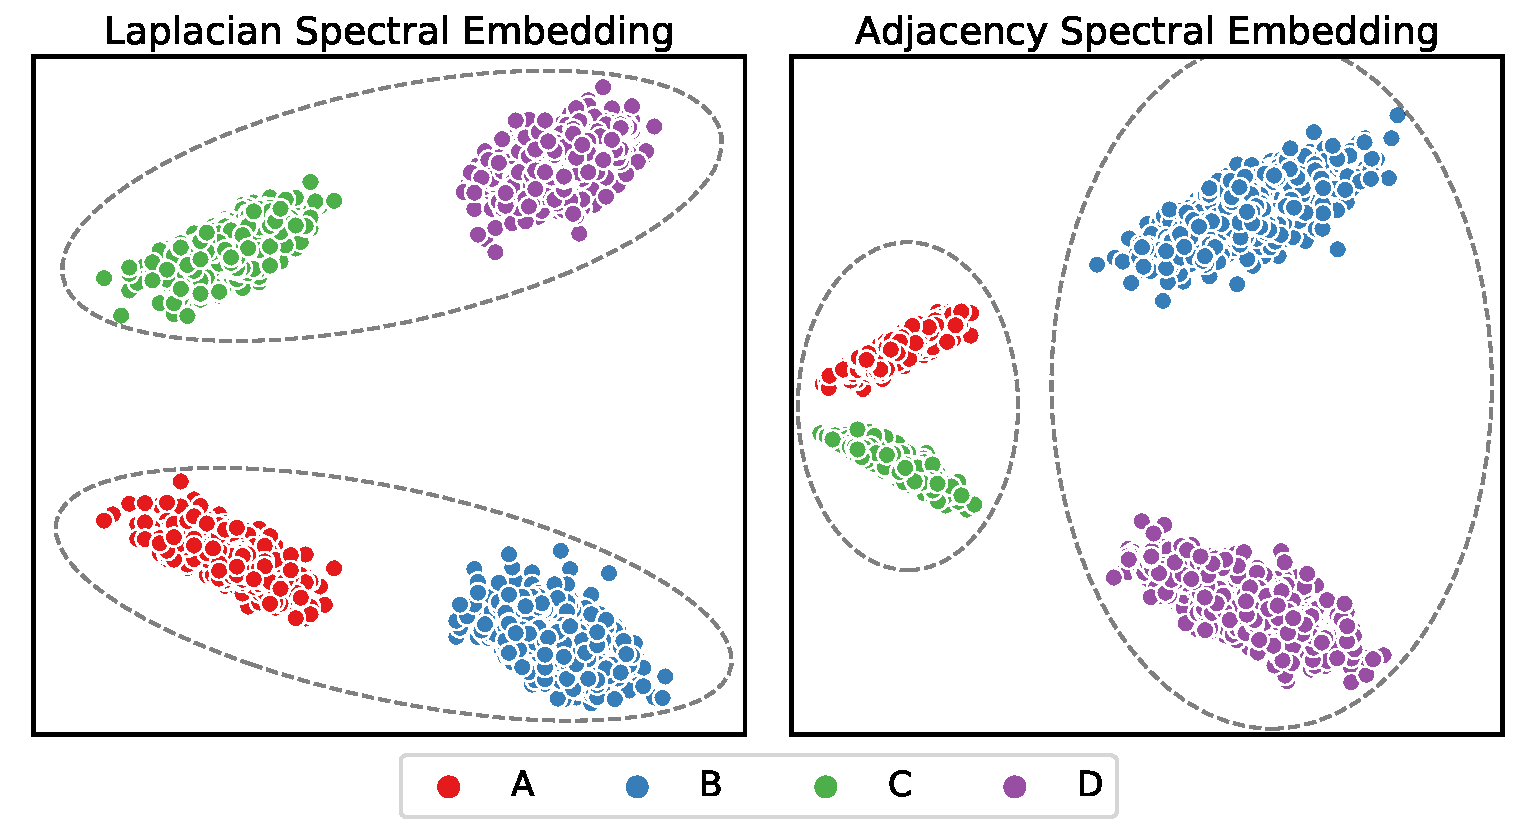
\includegraphics[width=0.7\textwidth]{figures/dnd/two_truths}
    \caption
    [Different clustering results from adjacency spectral embedding ($\ase$) and Laplacian spectral embedding ($\lse$).]
    {\textbf{Different clustering results from adjacency spectral embedding ($\ase$) and Laplacian spectral embedding ($\lse$).} For both $\ase$ and $\lse$, the network was embedded into $d=2$ dimensions, and Gaussian mixture modelling ($\gmm$) with $K=2$ clusters were fit. The dots represent vertices in the embedded space and the colors correspond to block memberships. The dashed black ellipses define the vertices that were clustered into same group.
    \textbf{a.} Clustering the embeddings from $\lse$ results in affinity clustering. 
    \textbf{b.} Clustering the embeddings from $\ase$ results in core-periphery clustering.}
    \label{fig:exp8}
\end{figure}

\subsection{Detecting Communities with Spectral Clustering}
Many of the techniques described above rely on knowing an \textit{a priori} grouping of nodes or edges, but in many real-world examples this information is not available. Additionally, one may seek to discover communities in the network, either for modeling the network as a block-model or to reveal groups of similar nodes. 

As described in Section \ref{sec:clustering_single}, one can embed a graph via $\ase$ or $\lse$ and then use $\gmm$ to reveal communities of nodes. Here, we separately embed both the left and right hemisphere induced subgraphs of the \textit{Drosophila} larva connectome using $\ase$ (see \cite{priebe2017semiparametric} for an extensive investigation) with $\hat d= 3$. $\gmm$ was performed independently on both hemispheres, with the clustering assignments and embeddings shown in Figure \ref{fig:mb-clustering}. Note that while the embedding and clustering of both hemispheres were performed separately, similar structures emerge for the left and right. In particular, each cluster is mostly comprised of a single cell type. Thus, spectral clustering can provide neuroscientists to find meaningful communities when the assignment is not known. 

\begin{figure}
    \centering
    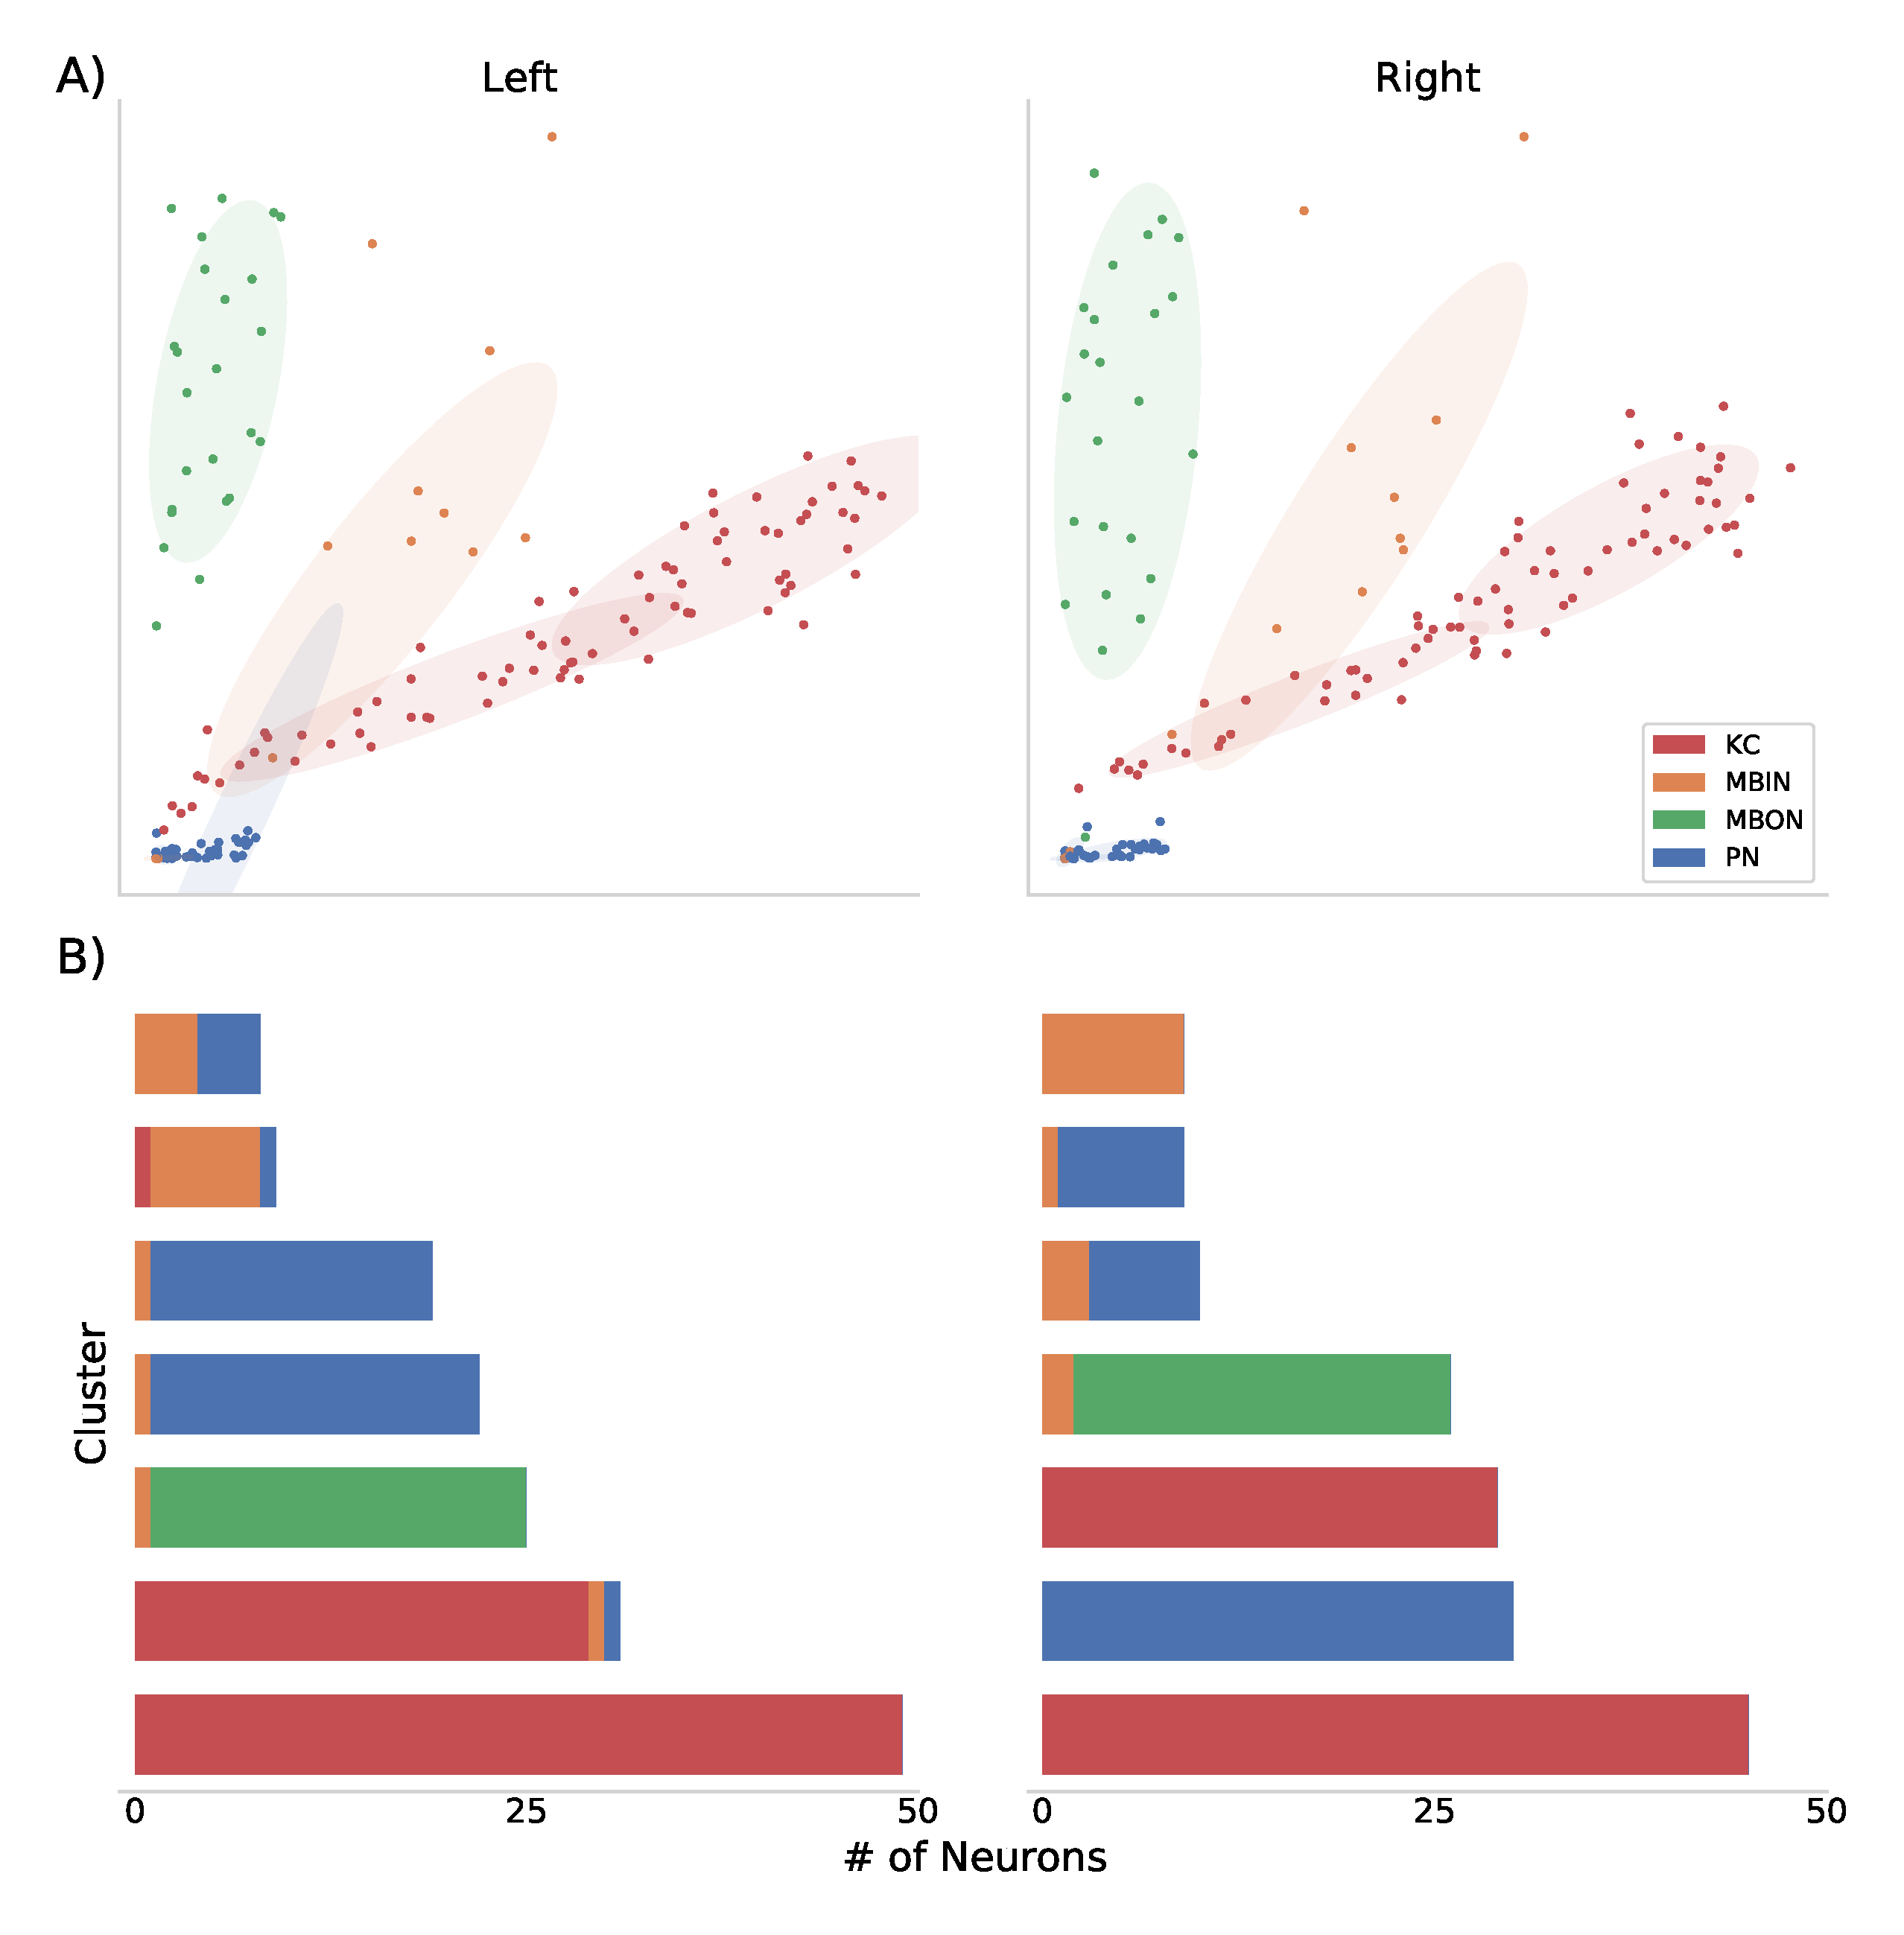
\includegraphics[width = .8\linewidth]{figures/dnd/mb-clustering.pdf}
    \caption
    [Spectral clustering of the \textit{Drosophila} mushroom body network.]
    {\textbf{Spectral clustering of the \textit{Drosophila} mushroom body network.} \textbf{a.} First ``in'' embedding dimension is plotted against the first ``out'' embedding dimension for both the left and right hemisphere networks (note that the clustering was performed in six dimensions, but only two are shown here for visualization). Each point represents a neuron, colored by its corresponding cell type. Ellipses show the clusters predicted by Gaussian mixture modeling, colored according to the cell type with the most frequent neurons in that cluster. Each color corresponds to one of Kenyon cells, input neurons, output neurons, and projection neurons. \textbf{b.} Stacked barplots showing each cluster's composition in terms of neuron cell type, for both the left and the right hemisphere clusterings. Each cluster is mostly comprised of a single cell type for both left and right hemisphere networks, meaning that spectral clustering can recover true communities. }
    \label{fig:mb-clustering}
\end{figure}

